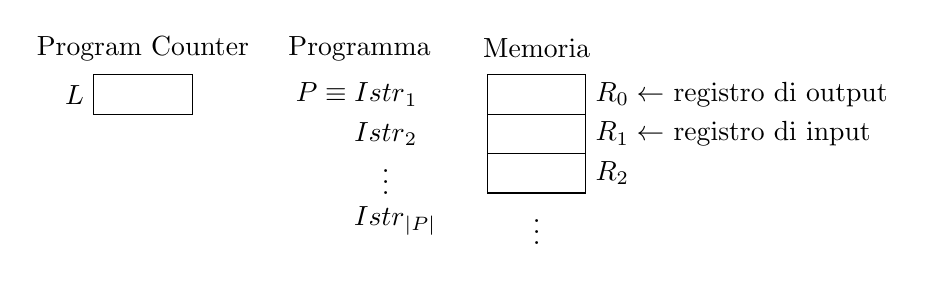
\begin{tikzpicture}
    \node[above] at (.875,.6) {Memoria};

    \draw (.25,0) rectangle (1.5,.5);
    \node[right] at (1.5,.25) {$R_0 \leftarrow$ registro di output};
    \draw (.25,-.5) rectangle (1.5,0);
    \node[right] at (1.5,-.25) {$R_1 \leftarrow$ registro di input};
    \draw (.25,-1) rectangle (1.5,-.5);
    \node[right] at (1.5,-.75) {$R_2$};
    
    \node[below] at (.875,-1) {$\vdots$};

    \def\y{2.25}
    \node[above] at (.875-\y,.55) {Programma};
    \node[] at (.84-\y,.25) {$P\equiv\text{Istr}_1$};
    \node[] at (1.21-\y,-.25) {$\text{Istr}_2$};
    \node[] at (1.21-\y,-.75) {$\vdots$};
    \node[] at (1.33-\y,-1.35) {$\text{Istr}_{|P|}$};

    \def\x{5}
    \node[above] at (.875-\x,.55) {Program Counter};

    \draw (.25-\x,0) rectangle (1.5-\x,.5);
    \node[left] at (1.5-1.25-\x,.25) {$L$};
\end{tikzpicture}
